\chapter{Resultados}
\label{chap:result}
Os robôs que atuam em mares, rios e lagos, também considerados como drone subaquático, estão ampliando cada vez mais as intervenções humanas nestes ambientes. Os objetivos das intervenções podem ser diversas, mas a industria de óleo e gás demandam a maior quantidade de aplicações destes robôs. 


%--------- NEW SECTION ----------------------
\section{Robôs Subaquáticos}

%Procurar algum artigo que possui definição de rovs
\label{underwater_robots}
De acordo com \cite{Bogue1}, Robôs Subaquáticos são importantes na industria petroelo, em ações militares e no monitoramento de ambiente. Estes robôs podem ser classificados em duas categorias diante do modo de operação. Os robôs que depedem de alguma intervenção humana, princiapalmente pela teleoperação, são classificados como remotely operated vehicles (ROVs)

Segundo \cite{Towards}, os ROVs são veículos subaquáticos que possuem um cabo para realizar comunicação e receber energia elétrica de alguma embarcação ou plataforma. Os ROVs podem ser classificados em três categorias: Eyeball ROV, Observation ROV e Work class ROV. Eyeball ROV, que tem como um dos principais elemetos uma câmera, são empregados geralmente para água razas, já os Observation ROV possui um tamanho maior e podem receber a implementação de manipuladores. Os Work class ROV são maiores, podem alcançar algumas toneladas e pode realizar ações complexas, assim como executar posicionamente dinâmico.

\subsection{Modelos de ROVs}

Existem vários modelos de robôs submarinos. O formato deste veículos podem ser em função de diversas considerações: local de atuação, profundidade onde as atividades serão executadas, suporte para a presença de braços manipuladores subaquático.

\subsubsection{BlueROV2}


O BlueROV2, representado na Figura \ref{fig:blue}, é desenvolvido pela Blue robotics, uma comphania americana especilizada em robô submarinos. Assim como informa \cite{Bluerobotics}, este veículo é destinado para realizar inpeções e pesquisas. O alcance de profundidade é de 100 m. 6 thursters são responsáveis pela atuação, 4 lâmpadas, também há versões com 6, e uma camêra HD coletar os dados visuais. 
Além destas configurações, outros intems pode ser adicionados ao exemplo de gripper, para realizar aconrragem, e sonares, para medição de profundidade e escananeamento. Um ponto importante do BlueROV2 é o fato de ROV ser opensource,  que permiti de várias modificações e dominio dos eventuais usuário.

\begin{figure}
  \centering 
  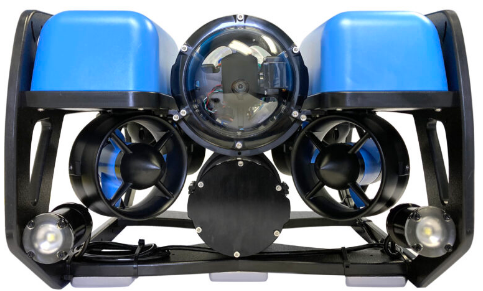
\includegraphics[width=150.5]{blue_rov.png}
  \caption{BlueROV2}
  \label{fig:blue}
\end{figure}

\subsubsection{Freedom ROV}


O Freedom ROV, apresentado na Figura \ref{fig:freedom_rov}, é desenvolvido pela comphania OCEANEERING, dentêm uma como a principal caracteristicas ter modos de operações híbridas. Segundo \cite{Bogue1}, Freedom pode operar sem intermédio de ações humanas, com ou sem a presença de cabos de comunicação. Este veículo também capacidade de realizar \textit{subsea residence}, que é capacidade dos robôs ficarem alocadod no mar por um perido longo, neste caso seis meses. Durante o periodo de residência submarina, o Freedom ROV realizar o recarregamento de energia em estações de docagem submersas.


\begin{figure}
  \centering 
  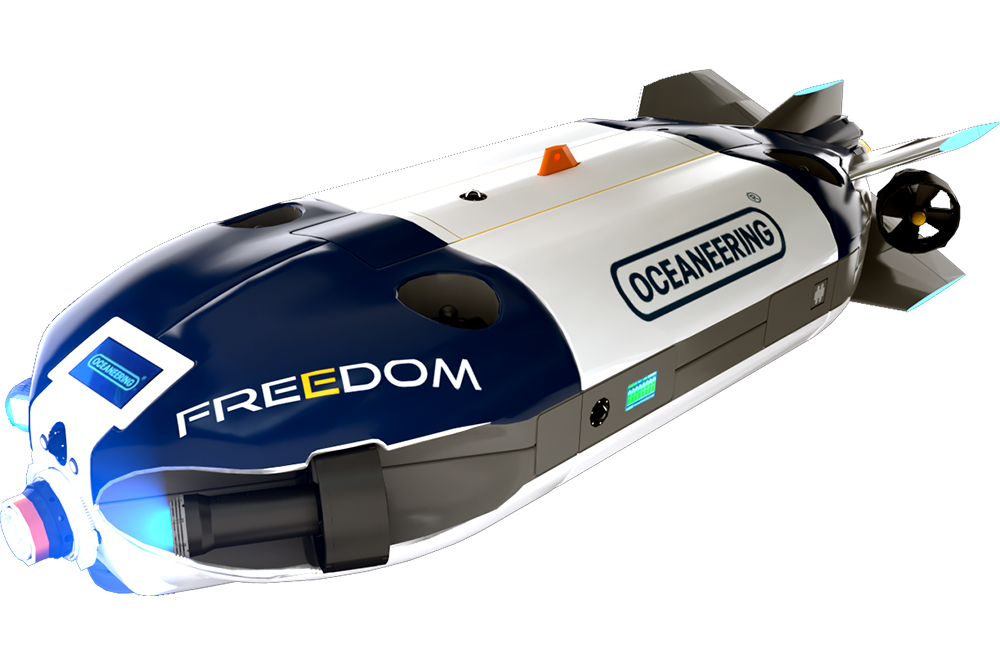
\includegraphics[width=150.5]{freedom_rov.png}
  \caption{Freedom ROV}
  \label{fig:freedom_rov}
\end{figure}

\subsubsection{SEASCAN MK2}


A ECA GROUP, uma companhia francesa especializada em desenvolver veículos marinhos e submarinos, desenvolveu um o ROV SEASCAN MK2, representado na Figura \ref{fig:seascan}. Este robô é tem uma forma de torpedo. De acordo com \cite{ECA_GROUP}, O SEASCAN é um veículo leve e pode ser usado para inspeções, identificação de minas e para missões com fins ambientais. Cabos umbilicais não são usados para nem para cominicação e nem para alimentação.  Uma bateria recarragável é a fonte de alimentação deste robô.

Também é apontado por \cite{ECA_GROUP} que o SEASCAN MK2 também pode realizar algumas duas tarefas autônomas. Uma é dedicada para realizar posicionamento diante a profundidade do veículo, a outra é focada em automatizar o caminho do veículo a alcançar uma area específica.



\begin{figure}
  \centering 
  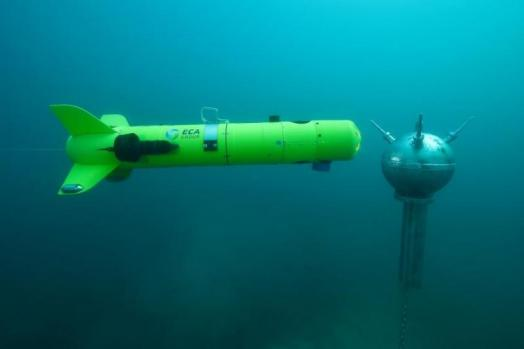
\includegraphics[width=150.5]{seascan.jpg}
  \caption{SEASCAN MK2}
  \label{fig:seascan}
\end{figure}


\subsubsection{Aquanaut ROV}

O Aquanaut ROV um é veículo, de acordo \cite{Bogue1}, que além de possuir operação hibrida, autonomo e teleoperado., também não possui um formato único. O Aquant ROV possui dois formatos de operação, um para o modo autonomo, e outro para realizar teleoperação.
A Figura \ref{aquanaut_auv} representa o Aquant na forma autonoma e  a Figura \ref{aquanaut_rov} é o foramto que o Aquant adiquiri ao passar para a atuação teleoperado.

O modo de atuação autonoma é realizada até o robô antingir o momento de realizar as atividades destinadas ao trabalhos com manipuladores. Para atuar de forma com os manipuladores, o Aquanaut mudar de formato e sua atuação passar a ser completamente por fins de teleoperação, em outras palavras há uma necessidade de presenaça  humana na operação. 


\begin{figure}
  \centering 
  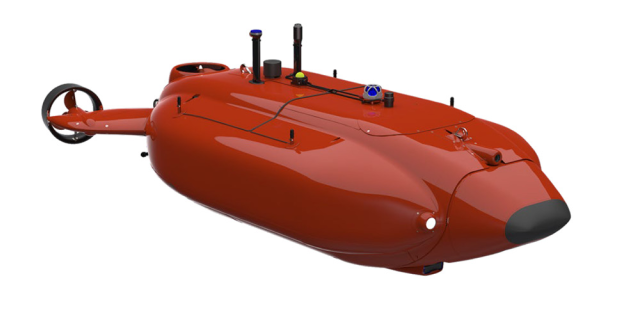
\includegraphics[width=150.5]{aquanaut_auv.png}
  \caption{Aquanaut em formato para realizar operações autonomanas}
  \label{fig:aquanaut_auv}
\end{figure}

\begin{figure}
  \centering 
  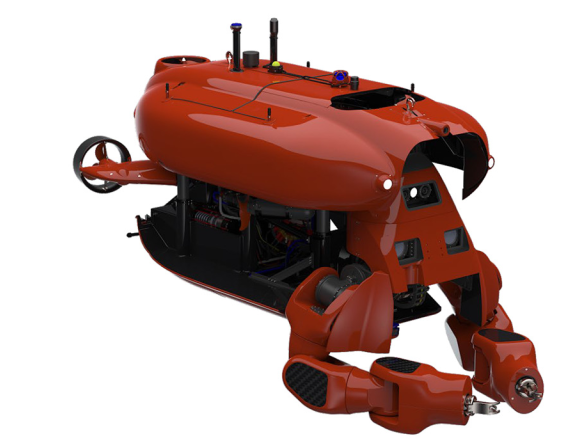
\includegraphics[width=150.5]{aquanaut_rov.png}
  \caption{Aquant em formato para teleoperação}
  \label{fig:aquanaut_rov}
\end{figure}



\subsection{Considerações na Modelagem}
Esta seção aborda os princiapis elementos e considerações para modelagens de ROVs.

Assim como quase todos robôs móveis podem estar posicionado em relação a uma referência, a posição de um robô subaquatico pode ser representando, de acordo com \cite{Antonelli}, diante a sua posição e orientação.
Diante a um Frame fixo de referência, é possivel obter a posição, usando técnicas de sensoriamentom, de um veículo submerso que comunalmente representando como vetor.
%vetor = (x,y,z)

Para representar a rotação dos veiculos diante ao mesmo frame pode usar o vetor
%n =(r,p,y)
que é a representação de roll, pitch  e yaw.

A seguinte tabela apresenta os movimentos dos veículos Subaquáticos em relação ao destes. Esta tabela esta de acordo que demostrado em \cite[Antonelli]. Estes movimentos, surge, sway e heave, também são usados navegações marinhas. Para acompanhar os movimentos dos ROVs sensores são comunalmente implementados nas estruturas destes.





%lembre de usar o livro de fossen
\subsection{Sensores}

A presença de sensores em um sistema pode permiti a obtenção de dados de vários. A medida dos sensores podem ser direcionados para a propria dinânica de um sistema, neste caso um ROV, e o ambinete no qual este realizar suas ações.
Assim como classifica \cite{Towards}, os sensores de um ROV pode distinguindo em dois grupos: \textit{playload sensors}  e \textit{navigations sensor}. Os \textit{payload sensors} são unidades de medidas destinados a coletar dados do ambiente, alguns exemplos destes sensores saão: sensores CTD, destinados a mensurar a condutividades, temperatura e profundidade, sensores ADCP-Acoustic Doppler Curent pPofiler- são usados para mensurar a velocidade das correntes e câmeras para obter dados visuais.

Os navigations sensors são implementados com o foco na navegação do veículo, logos dados sobre a posição, orientantçã e veocidade são os principais alvos a serem mensurados. Os navigations sensors mais comum são: sensores de pressão, (DVL) mede o deslocamento Doppler no sinal de entrada refletido no fundo do mar para obter os dados da velocidade linear e sensores de inercia. 
Câmeras também podem ser usadas para obter dados da posiação de veículos, assim como foi demostrado por \cite{visual_serving}, no qual foi ultizado duas câmeras par realizar um acomphamento da posição de ROV. Os dados dos sensores podem ser usados para o monitoramento e para as ações de controle.
% lembrar de falar sobre o %USBL
% Colocar a tabela com as imagens dos principais sensores
%USBL



\subsection{Controle}
% tipo de controle
% desenhar no drawio um esquematico dos controles para rovs
Para os ROVs, grande parte do objetivo do contole é focado na movimentação. A aplicação de   estratégia de  controle linear tem forte presença. \cite{Towards} afirma que os controles de movimentos que constumam ser aplicado em ROV são direcionados para desenvolver capacidade de manejo e acomphamento de profundidade. No veículo DexROV, \cite{desgin_joy} implentou aplicou controle em  seis funcionaliades de movimentos, são estes: \textit{Hovering} - posição dinâmica, \textit{Autodepth} controle de profundidae, \textit{autoheading} controle de direção, \textit{autoaltitude} controle de altitude e \textit{Guidance to target position}. Para cada funcionalidade, foi implementada controle proporcional intregal usando dados de USBL. Mesclando o uso destas funcionaliades, com a desconsideração  da existências de obstacuslos, pode ser possivel implementar uma navegação do DexROV.

Uma aplicação de um controle PID não-linear foi aplicado por \cite{wireless_joy}. A aplicação foi destinada para realizar um modo de auto-piloto para ROV.

Para obter dominio sobre uma  desejada posição, \cite{visual_serving} implementou a estratégia de controle proporcional. A estimação da posição do ROV foi obtida usando algortimo genético em dados captados por um câmera dual. O resultado da implementação foi suficiente para vencer pertubações sofridas pelo o veiculo em diferentes posições. A aplicação de controlr proporcinal não é muito complexa, mas gerou bons resultados que também foi devida a acuricidade da estimação da posição que foi por volta de +- 20 mm. 
Em outra aplicação apresenta por \cite{dual_eyes}

Para controle de posicionamento de veiculos subaquaticos, esta estratégia atende muito bem, mas para uma operação que requer uma maior precisão das variaveis desejadas, ao exemplo controle de trajetoria de manipuladores, talvez uma aplicação mais robusta pode prover um resultado melhor.  

% objetivo de controle

\subsection{Atuação}
% Thrusters
%% Tipo de Thrusters
%Fins
% Tipos de Fins

\subsection{Arquitetura de Operação}
Há diversas formas que as arquiteturas de operação diante do nível de autonomia dos ROVs podem ser implementados. Uma comum é quando um humano é responsável 100\% das atuações do veículos, em outras palavras, é aplicado um controle 100\% manual. O operador, neste caso costuma ser um bastante habilidoso, comunalmente usa uma video câmera para estimar a posiação do veículo no ambiente. \cite{Towards} aponta que uma estrátegia para o controle manual é ultilizar um Head-Mounted display (HMD) juntamente com um joytsick. A ultilização do HMD é dedicado para a navegação do veículo, enquanto o joystick pode ser empregado para operar os braços manipuladores.
% achar uma referência para o controle manual.

Uma arquitetura, segundo \cite{wireless_joy}, é \textit{Human in the Loop} - HITL- que é realizado considerando a arquitetura \textit{Human Centered Automantion} - HCA. Nesta arquitetura o operador humano realizar algumas tarefas do sistema de controle, ao exemplo de selecionar de qual mode de ação de movimento o veiculo deve realizar. Alguns exemplos dos modo de ação o controle de profundidade, heading e seguir tubulações.

Outros tipos de operações são apontadas por \cite{Towards}: \textit{Automatic Operation}, \textit{Management by consent}, \textit{Semi-autonomous or management by exception} e \textit{Highly autonomous}. O primeiro, \textit{Automatic Operation}, possui caracteristicas semelhante ao \textit{human in the loop} e o segundo, \textit{Management by consent} é basicamente uma teleoperação. O \textit{Semi-autonomous or management by exception} é montado para o sistema executar automaticamente as funções relacionadas à missão quando os tempos de resposta são muito curtos para intervenção humana.  Quando não necessidade de um operador realizar nenhuma intervenção sobre o veiculo, o tipo de operação é considerada \textit{Highly autonomous}. Esta última classificação esta mais proxima das condicções necessarios para um veículo submarino ser considerado um AUV. As estruturas de operação podem variar em função das atividades que os ROVs realizam e também considera os modelos destes. 








%--------- NEW SECTION ----------------------


\section{Revisão bibliográfica}
\subsection{Rede de Citação}
\subsection{Principais autores}

%--------- NEW SECTION ----------------------

\section{Mapa COnceitual}
\lipsum[1]

%--------- NEW SECTION ----------------------






